% Giacomo Petrillo
% lezione di Punzi

\subsection{Robustezza}

Fino a ora ci siamo occupati di ottimizzare uno stimatore per un certo modello,
cioè dell'\emph{incertezza statistica}.
Tuttavia può essere utile tener conto dell'\emph{incertezza sistematica},
cioè del comportamento su più modelli.
La questione di quanto continui a funzionare bene uno stimatore se cambiamo modello è detta \emph{robustezza}.

\begin{example}
	Il Particle Data Group\footnote{Vedi \url{http://pdg.lbl.gov/2017/reviews/rpp2017-rev-rpp-intro.pdf}, §5.2.2.}, quando deve combinare più misure, usa la media pesata\footnote{Vedi \autoref{th:wavg}.}, tuttavia stima la varianza della media pesata in modo non standard.
\end{example}

\begin{example}
	Abbiamo visto che la varianza campione
	\begin{equation*}
		\hat\sigma^2_A \is \frac1N \sum_i (x_i-\bar x)^2
	\end{equation*}
	ha un bias che non dipende dalla distribuzione e,
	nel caso della gaussiana,
	è una statistica sufficiente e lo stimatore di massima likelihood.
	Inoltre probabilmente il lettore l'avrà già incontrata e avrà imparato a usarla abitualmente.
	Tuttavia un tempo non era scontato usare la varianza campione,
	l'alternativa principale era la media degli scarti
	\begin{equation*}
		\hat\sigma_B \is \frac1N \sum_i |x_i - \bar x|
	\end{equation*}
	come stima della deviazione standard.
	Il bias dipende dalla distribuzione, nel caso della gaussiana si ottiene
	\begin{equation*}
		E[\hat\sigma_B] = \sqrt{\frac2\pi} \sigma.
	\end{equation*}
	Chiamiamo $r$ il rapporto asintotico tra le varianze dei due, fissata una qualche distribuzione:
	\begin{equation*}
		r \is \lim_{N\to\infty} \frac {\var[\hat\sigma_A]} {\var\left[\sqrt{\frac\pi2}\hat\sigma_B\right]},
	\end{equation*}
	nel caso della gaussiana si ottiene $r=0.876$.
	Ci fu un dibattito tra Fisher e Eddington su quale fosse nella pratica il migliore dei due,
	Fisher ebbe ragione per il fatto che $r<1$.
	Tuttavia in seguito $\hat\sigma_B$ venne riconsiderato per la maggiore robustezza.
	Consideriamo ad esempio la gaussiana ``con code maggiorate''
	\begin{align*}
		p(x;\mu,\sigma)
		&= (1-\epsilon)\cdot g(x;\mu,\sigma) + \epsilon\cdot g(x;\mu,3\sigma) \\
		\text{dove }g(x;\mu,\sigma)
		&\is \frac1{\sqrt{2\pi}\sigma} \exp \left(-\frac12\left(\frac{x-\mu}\sigma\right)^2\right)
	\end{align*}
	(quindi qui $\sigma$ non è la deviazione standard della distribuzione).
	Una distribuzione del genere può essere ad esempio un modello per la presenza di \emph{outliers}.
	Vediamo come varia $r$ all'aumentare di $\epsilon$:
	\begin{center}
		\begin{tabular}{ll}
			$\epsilon$ & $r$ \\
			\hline
			0     & 0.88 \\
			0.001 & 0.95 \\
			0.002 & 1.01 \\
			0.05  & >2   \\
		\end{tabular}
	\end{center}
	Intuitivamente la ragione è che il quadrato è più sensibile a valori che si allontanano dal centro.
\end{example}

Generalizziamo l'espressione a un esponente arbitrario:
\begin{align*}
	\hat\sigma_p
	&\is \left(\frac1N \sum_i (x_i - \hat m_p)^p\right)^{1/p}
\end{align*}
dove $\hat m_p$ è definito come quello che minimizza l'espressione.

\paragraph{Moda campione}

Nel limite $p\to-\infty$ gli scarti che contano nella somma sono quelli più piccoli,
quindi posso trovare $\hat m_{-\infty}$ con questa procedura:
prendo i due $x$ più vicini tra loro, poi dei due scelgo quello il cui secondo vicino è più vicino.
$\hat m_{-\infty}$ è la \emph{moda campione} e in effetti stima bene la moda.
La moda è utile per le distribuzioni che non hanno media definita,
ad esempio la distribuzione di Landau.

\paragraph{Semidispersione}

Per $p\to\infty$ contano gli scarti più grossi,
quindi si ottiene
\begin{align*}
	\hat m_\infty
	&= \frac{\min\mathbf x + \max\mathbf x}2 \\
	\hat\sigma_\infty
	&= \frac{\max\mathbf x - \min\mathbf x}2
\end{align*}
che sono rispettivamente \emph{midrange} e \emph{semidispersione}.
\begin{example}
	Consideriamo la distribuzione uniforme con media $\mu$ e larghezza $m$:
	\begin{equation*}
		p(x;\mu,m)
		= \frac1m \chi_{(\mu-m/2,\mu+m/2)}(x).
	\end{equation*}
	La likelihood per $N$ estrazioni è
	\begin{equation*}
		p(\mathbf x;\mu,m)
		= \frac1{m^N} \chi_{(\mu-m/2,\infty)}(\min\mathbf x) \chi_{(-\infty,\mu+m/2)}(\max\mathbf x).
	\end{equation*}
	Calcoliamo lo stimatore di massima likelihood.
	Dobbiamo massimizzare $m^{-N}$ scegliendo un intervallo con centro $\mu$ e larghezza $m$ che contenga $\mathbf x$,
	ovvero l'intervallo di larghezza minima.
	Quindi $\hat\mu=\hat m_\infty$, $\hat m=2\hat\sigma_\infty$.
\end{example}

\paragraph{Mediana campione}

Consideriamo il caso $p=1$.
Siano $N_-$ gli $x_i$ minori di $\hat m_1$ e $N_+$ quelli maggiori.
Se traslo $\hat m_1$ di $\Delta x$ abbastanza piccolo in modo da non cambiare $N_+$ e $N_-$,
la somma degli scarti cambia di $\Delta x(N_- - N_+)$.
Quindi il minimo si ha per $N_+ = N_-$.
L'astuto lettore avrà riconosciuto che $\hat m_1$ è la \emph{mediana campione}.
Nel caso di $N$ pari il minimo non è unico e per convenzione si sceglie la media dei due $x_i$ centrali.
Nel caso di $N$ dispari il minimo è l'$x_i$ centrale.
\begin{fact}
	La mediana campione è una stima consistente della mediana.
	\marginpar{Non abbiamo definito la mediana.}
\end{fact}
La mediana non è definita per tutte le distribuzioni (vedi ad esempio \autoref{fig:nomedian}),
perché la cumulante di una distribuzione non è in generale strettamente crescente.
\begin{figure}
	\centering
	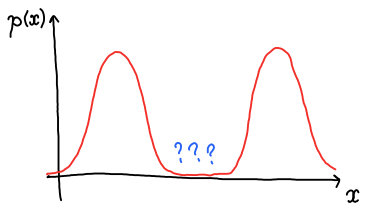
\includegraphics[width=17em]{nomediana}
	\caption{\label{fig:nomedian}%
	Distribuzione di probabilità che non ha una mediana definita.}
\end{figure}
La mediana e la mediana campione,
a differenza della media,
trasformano banalmente per cambiamento di variabile.
Inoltre la mediana campione (e quindi anche la mediana) ha la proprietà che non dista dalla media più di una deviazione standard:
\begin{align*}
	|\mu-\hat m_1|
	&= |E[x-\hat m_1]| \le \\
	&\le E[|x-\hat m_1|] \le \\
	\intertext{(per definizione di $\hat m_1$)}
	&\le E[|x-\mu|] \le \\
	&\le \sqrt{E[(x-\mu)^2]} = \sigma.
\end{align*}
Si dimostra anche che:
\begin{align*}
	|\bar x - \hat m_1|
	&\le \sqrt{\frac35}\,\sigma, \\
	|\hat m_{-\infty} - \hat m_1|
	&\le \sqrt3\,\sigma.
\end{align*}
Calcoliamo la pdf della mediana campione.
Consideriamo per semplicità il caso $N$ dispari:
allora la mediana campione è il campione centrale.
La probabilità è la probabilità del campione per la probabilità che sia il campione centrale;
calcoliamo quest'ultima.
Definito
\begin{equation*}
	k \is \frac{N-1}2,
\end{equation*}
la probabilità che il campione centrale sia centrale è
la probabilità che i $k$ minori siano minori
per la probabilità che i $k$ maggiori siano maggiori
per il numero di permutazioni degli altri campioni in cui il campione centrale rimane centrale,
cioè il numero di modi in cui posso estrarre due insiemi di $k$ elementi da uno di $N$,
che è dato dal coefficiente multinomiale
\begin{equation*}
	\frac{N!}{k!k!1!}.
\end{equation*}
Detta $p_x$ la pdf di $x$ e $F$ la cumulante, infine
\begin{equation*}
	p(\hat m_1)
	= p_x(\hat m_1)
	\cdot F(\hat m_1)^k
	\cdot \big(1-F(\hat m_1)\big)^k
	\cdot \frac{N!}{(k!)^2}.
\end{equation*}
\begin{example}
	Scriviamo la distribuzione della mediana campione per la distribuzione di Cauchy:
	\begin{align*}
		p_x(x)
		&= \frac1\pi \frac1{1+x^2} \\
		F(x)
		&= \frac1\pi\arctan x + \frac12 \\
		p(\hat m_1)
		&= \frac 1\pi \frac1{1+\hat m_1^2}
		\cdot \left(\frac12 - \frac1\pi\arctan(\hat m_1)\right)^k
		\cdot \left(\frac12 + \frac1\pi\arctan(\hat m_1)\right)^k
		\cdot \frac{N!}{(k!)^2} \propto \\
		&\propto \hat m_1^{-(k+2)} + O\big(\hat m_1^{-(k+4)}\big) \text{ per $\hat m_1\to\pm\infty$},
	\end{align*}
	quindi la mediana campione ha varianza definita per $k\ge2$ ovvero $N\ge5$.
\end{example}

\begin{fact}
	La varianza asintotica della mediana campione è
	\begin{equation*}
		\var[\hat m_1]
		= \frac1{4p_x^2\big(F^{-1}(1/2)\big)}\frac1N + O\left(\frac1{N^2}\right).
	\end{equation*}
\end{fact}

\noindent Notiamo che la varianza asintotica non dipende dalla varianza della distribuzione di $x$,
infatti non è necessario che sia definita.

\begin{exercise}
	\marginpar{Ho letto in rete delle dimostrazioni che usano la cumulante empirica ma non le ho capite.
	Sia $F_{\mathbf x}$ la cumulante empirica,
	le dimostrazioni dicono che la variabile $F^{-1}(F_{\mathbf x}(F^{-1}(1/2)))$
	ha la stessa distribuzione della mediana campione $F_{\mathbf x}^{-1}(1/2)$,
	ma non capisco perché. \\
	\emph{Sul Del Prete alle pagine 159--160 c'è una dimostrazione con lo sviluppo in serie.}}
	Dimostrare che la distribuzione asintotica della mediana campione è gaussiana.
\end{exercise}

\begin{exercise}
	Trovare una distribuzione tale che la stima di massima likelihood per la media è la mediana campione.
\end{exercise}

\begin{solution}
	La mediana campione è definita come il $\mu$ che minimizza
	\begin{equation*}
		\frac 1N \sum_i |x_i - \mu|;
	\end{equation*}
	se imponiamo che la likelihood sia una funzione monotona descrescente di questa espressione,
	la stima di massima likelihood sarà uguale alla media campione.
	Tuttavia vogliamo anche che la likelihood sia il prodotto di termini $p(x_i;\mu)$,
	la somma sugli~$i$ suggerisce di considerare l'espressione come il logaritmo della likelihood:
	\begin{align*}
		\log p(\mathbf x;\mu)
		&= -\sum_i |x_i - \mu| + C \implies \\
		\implies p(x;\mu)
		&= \frac12 e^{-|x-\mu|}.
	\end{align*}
\end{solution}

\paragraph{Medie troncate}

Consideriamo ora la robustezza della media aritmetica.
Se come modelli consideriamo quelli con code maggiorate,
il modo più semplice di rendere la media aritmetica più robusta è eliminare i campioni più esterni.
Questa procedura si chiama \emph{media troncata}.
Sia $k$ il numero di campioni che eliminiamo a destra e a sinistra,
definiamo
\begin{equation*}
	r \is \frac12 - \frac kN.
\end{equation*}
Per $r=1/2$ riotteniamo la media aritmetica mentre per $r=0$ si ha la mediana campione.
Un'altra possibilità è la \emph{media winsorizzata},
cioè i due campioni estremi rimasti dopo averne eliminati $k$ a destra e a sinistra vengono pesati con $k$.
Si ottiene che $r=0.22$ è un buon valore da usare e che la media winsorizzata funziona peggio di quella troncata.
\marginpar{Questa parte sul 0.22 etc è vaga. Come è fatto il test?}%

